\documentclass[12pt, a4paper,twoside]{report}

%% Every LaTeX document begins with a preamble, which loads packages and defines various
%% settings to make the document look right. Mostly, you can ignore everything in this
%% template before \begin{document} on line 74

\usepackage{mathtools,amsthm,amsfonts} % Enable useful mathematical symbols/environments
\usepackage{graphicx} % Enable graphics
\usepackage{fancyhdr,titlesec,microtype} % enable various formatting commands
\usepackage[margin=2.5cm]{geometry} % Set margin size
\usepackage{palatino} % Set the font
\usepackage[latin1]{inputenc} % Allow you to input accents, umlauts and other characters
\usepackage[T1]{fontenc} % Lets LaTeX print a wider array of characters
\usepackage{tikz,tikz-3dplot,tkz-euclide} % Enable tikz drawings

\usepackage{xcolor} % Enable coloured elements
\definecolor{mypurple}{HTML}{622567} %%% Purple
\definecolor{myred}{HTML}{D55C19} %%%EssexOrange
\definecolor{myblue}{HTML}{007A87} %%%Seagrass

% For technical reasons, hyperref should be loaded after all other packages
\usepackage[colorlinks,linkcolor=myblue,citecolor=mypurple]{hyperref}

\renewcommand{\baselinestretch}{1.5} % 1.5 line spacing

% Define \begin{theorem}, \end{theorem}, etc.
\theoremstyle{plain} % The following environments will be italicised
\newtheorem{theorem}{Theorem}[chapter]
\newtheorem{lemma}[theorem]{Lemma}
\newtheorem{proposition}[theorem]{Proposition}
\newtheorem{corollary}[theorem]{Corollary}

\theoremstyle{definition} % The following environments will not use italics
\newtheorem{definition}[theorem]{Definition}
\newtheorem{example}[theorem]{Example}

\theoremstyle{remark} % The following environments will not use italics or bold titles
\newtheorem{remark}[theorem]{Remark}

\numberwithin{equation}{chapter}

% Fancy headings
\setlength{\headheight}{15pt}
\pagestyle{fancy}
\fancyheadoffset[LE,RO]{0pt}
\renewcommand{\chaptermark}[1]{\markboth{#1}{}}
\renewcommand{\sectionmark}[1]{\markright{\thesection\ #1}}
\fancyhf{}
\fancyhead[LE]{\makebox[0pt][l]{\thepage}\hfill\leftmark}
\fancyhead[RO]{\rightmark\hfill\makebox[0pt][r]{\thepage}}
\fancypagestyle{plain}{%
    \fancyhead{} % get rid of headers
    \renewcommand{\headrulewidth}{0pt} % and the line
}

% Fancy chapter numbers
\titleformat{\chapter}[display]
    {\normalfont\bfseries\color{myred}}
    {\filleft\hspace*{-60pt}%
        \rotatebox[origin=c]{90}{%
            \normalfont\color{black}\Large%
            \textls[180]{\textsc{\chaptertitlename}}%
        }
        \hspace{10pt}%
        {\setlength\fboxsep{0pt}%
            \colorbox{myred}{\parbox[c][3cm][c]{2.5cm}{%
                \centering\color{white}\fontsize{80}{90}\selectfont\thechapter}%
            }
        }
    }
    {10pt}
    {\titlerule[2.5pt]\vskip3pt\titlerule\vskip4pt\LARGE\sffamily}

\begin{document} % Start your document

%%%%%%%%%%%% BEGIN TITLE PAGE %%%%%%%%%%%%

\thispagestyle{empty} % For the title page, no header / footer

\noindent
    \begin{minipage}{0.1\textwidth}
    
\includegraphics[width=0.35\textwidth]{essex.png}
    \end{minipage}
    \begin{minipage}{0.89\textwidth}
    % \begin{center}
        \renewcommand\familydefault{\sfdefault}
        \fontfamily{phv}\selectfont
        {\Large \bf \sl University of Essex}\\[0.7em]
        {\Large \bf Department of Mathematical Sciences}
    % \end{center}
    \end{minipage}

\begin{center}
    \noindent\textcolor{myred}{\rule{\linewidth}{4.8pt}}
    
    \vspace{2em}
    \noindent {\LARGE \sc MA981 Dissertation}
    
    \vspace{3em}
    \noindent {\Huge{\color{myblue} Identification of brain tumour from brain MRI image using machine learning techniques}}
    
    \vspace{3em}
    \noindent {\Large \bf Pranav Patel \\ Registration number : 2207273}
    
    \vfill
    \noindent {\Large {Supervisor:} {\color{mypurple} \bf Danilo Petti}}
    
    \vspace{0.5em}
    \noindent\textcolor{myred}{\rule{\linewidth}{4.8pt}}
    
    \vspace{2em}
    {\Large \today }
    
    {\Large Colchester}
\end{center}

\clearpage

%%%%%%%%%%%% END TITLE PAGE %%%%%%%%%%%%

\tableofcontents

% If you have lots of figures with captions / numbers, uncomment the following line
\listoffigures

% If you have lots of tables and want a list of them, uncomment the following line
\listoftables

\chapter{Introduction}\label{ch:1}
The bulk of the human central nervous system(CNS) consists of the brain and the spinal cord.CNS's vital component, the brain is essential for controlling a variety of bodily processes, including analysis, decision-making , organisation, integration, and most importantly transmitting message throughout the body. The CNS of human being has very complex anatomical structure. Unfortunately, there are several reasons which can directly affect CNS, including headaches, infections, brain tumours, and stroke, present major difficulties for identification, investigation, and the creation of efficient treatments \cite{arabahmadi22}. Abnormal growth of cells and tissues inside the brain is the main cause of brain tumors. Having a tumor inside the skull is a concern as it can cause damage to the brain. The precise signs and symptoms of brain tumours, as well as their underlying causes, are currently unknown. As a result, people may have brain tumours without realising the seriousness of their condition. A tumor is classified as either malignant (cancerous)  or benign (non-cancerous)  depending on shape, location, and texture \cite{mabray15}. Particularly malignant tumours develop quickly in the brain, harming healthy tissues and having the potential to metastasize to other body organs \cite{lakshmi22}. Brain tumor ranks in tenth place for cause of deaths in children and grown person\cite{iorgulescu22}. If not discovered at the early stage, the survival rate is significantly less for this type of tumor.

According to the American Cancer Society, brain tumours are dangerous conditions marked by abnormal growth of brain tissue that impairs brain function. Brain tumors are traditionally classified as; (1) Slow-growing tumors: These tumours have a slow rate of spreading and take time to form. 
this type of tumor can be substantially eradicated by surgical procedure and are related to a higher risk of well-defined borders. An illustration of such a tumour is a pilocytic astrocytoma. (2) Progressive tumors: These tumours grow slowly over time, despite the fact that they might invade the tissues around them and advance to higher grades. Even while receiving continued treatment, these tumours can be found. An example of a tumour that advances in size is an oligodendroglioma. (3) Faster-growing tumors: Compared to type 2 malignancies, these tumours develop more quickly and have higher possibility to spread through the close by tissues. Surgical procedures alone cannot cure this type of tumor hence, it is constantly treated with radiation or post-operative chemotherapy. An example of a tumour that grows more quickly is anaplastic astrocytoma. (4) Highly malignant tumors: These types of tumours are the most aggressive and are more likely to spread. Even blood vessels can be used by them to promote growth. A particularly dangerous tumour is glioblastoma multiforme \cite{lundervold19}.

The (NBTF) which stands for National Brain Tumour Foundation reports that the number of brain tumor-related deaths has significantly increased by 300\% during the last three decades \cite{el14}. It is certain that every year  people around 250,000 suffer from brain tumour out of which 2\% comprises of cases with malignancies \cite{tiwari22} among the United States, 13,590 men and 10,300 women were expected to be diagnosed with a brain tumour among adults in 2020, totalling 23,890. The same year, 1,879 cases of brain cancer were recorded in Australia. Every year in America the case of primary brain tumour accounts for 14.1\%, with children accounting for 70\% of these occurrences. Primary brain tumours do not now have an early therapy, although over long period of then the cause negative repercussions \cite{anaya22}. Notably, there has been a considerable rise in brain tumour cases worldwide between 2004 and 2020, rising from around 10\% to 15\% \cite{xie22}. The complexity of brain tumours makes diagnosis and patient care difficult for medical professionals. Early diagnosis of brain tumours and fast treatment initiation are essential for increasing these patients' survival rates \cite{mcfaline22}. Finding non-invasive ways to accurately diagnose brain tumours is crucial because, unlike biopsies of other body areas, brain tumour biopsies necessitate surgical treatments. 

Tumour removal and early identification are essential for preserving the life of patients suffering from tumour. MRI (Magnetic Resonance Imaging) is an essential method in identifying, treatment, and follow-up of brain tumours. Although, MRI scan is a skillful, time consuming, and the analysis process id quite complex. The results of manual tumour identification can vary depending on the clinical specialists' experience and are particularly challenging. There are many difficulties in effectively classifying and segmenting MRI images. The goal is to construct an proficient infrastructure that aids in the precise treatment of malignant cells in brain MRI scans in order to address this problem. By assuring early intervention and suitable treatment, this approach would be a great help in overcoming the difficulties in diagnosing cancer of brain. Detection of brain tumour cells has been done by researchers from several fields over the years using image recognition algorithms. They have used numerous machine learning (ML) algorithm and deep learning (DL) algorithm are employed to identify malignant cells when it is in its early stage. Brain tumours must be promptly identified and accurately classified in order to guarantee effective care and enhance patient outcomes. However, due to a number of characteristics, including their different shapes, sizes, appearances, locations, scanning settings, and modalities \cite{lundervold19}, the diagnosis of brain tumours poses major hurdles. This task is handled by combining conventional and sophisticated methods. For identifying lesions, conventional techniques like radioactive beams, Gamma Knife (GK), and  Leksell Gamma Knife are frequently utilised. These techniques, however, frequently involve people and can be time-consuming \cite{rundo16}.

Brain tumour detection uses a various methods which involves medical imaging such as Positron Emission Tomography (PET), Magnetic Resonance Imaging (MRI), and Computer Tomography (CT). A special MR method known as chemical exchange saturation transfer (CEST) also enables image compounds at concentrations that are too low to have an impact on the contrast of traditional method MR imaging or to be clearly distinguished in Magnetic Resonance Spectroscopy (MRS) at ordinary water imaging resolution. Among these techniques, MRI scans are particularly useful since they provide a noninvasive way to visualise inside body structures using magnetization and microwave pulses. The Three types of patterns which involves magnetic resonance image to diagnose brain tumours are  T1 weighted, Fluid Attenuated Inversion Recovery (FLAIR),and T2 weighted. It is extremely difficult to accurately identify and detect tumor or infected regions using brain MRI. Due to the MRIs' increased complexity, humans are not capable to recognise minute alterations through their visual system. Therefore, researchers have created computer aided diagnostic (CAD) tools for radiologists which assists them in providing correct treatment \cite{rundo16}. Leksell Gamma Knife is a useful method for tumour diagnosis, although the presence of brain necrosis can compromise its accuracy. As a result, utilising efficient machine learning techniques is crucial to solving this problem.

Recent developments in machine learning have made it easier to recognise and categorise patterns in medical imaging. Notably, these developments allow for the direct extraction and retrieval of knowledge from data, which lessens the need for specialists or academic literature. In a number of medical applications, such as disease prognosis and diagnosis, detection of structure of cellular and molecular form, seperation of tissue, and categorization of picture, machine learning is proving to be an invaluable tool for improving performance \cite{militello15}. Currently, Convolutional Neural Networks (CNNs) happens to be the best effective methods for image accuracy and have several layers \cite{juan15}. By integrating a Random voxel clustering technique with Forest classifier, \cite{bonte18} has developed a revolutionary approach. Similar to this, \cite{militello15} have developed a semi-automated technique that accurately segments lesion volumes using an unsupervised FCM clustering algorithm in an effort to circumvent the lengthy nature of traditional diagnosis procedures like the Leksell Gamma Knife. \cite{xie22} have suggested a pipeline for segmenting brain tumours that combines four algorithms (K-means, Fuzzy K-means, Gaussian Mixture Model, and Gaussian Hidden Markov Random Field). Multispectral MRI data are not required thanks to the two-stage mechanism for dose escalation assessment that is presented in \cite{rundo18}. They include the FCM algorithm in their architecture and present NeXt, a fully automatic necrosis extraction technique.

While deep learning models have been adopted in order to achieve increased performance, machine learning (ML) approaches have been demonstrated successful in reliably detecting tumour locations in MRI images due to the availability of complicated, voluminous data and high-speed computing systems. The necessity for computer-assisted therapies is highlighted by the dependence on the expertise of human radiologists, the possibility of errors due to differences in pathology, and the weariness of human radiologists. Medical professionals can use computational intelligence-based tools to help them recognise and categorise brain tumours. With a focus on brain tumours, machine learning model is essential for the analysis, segmentation, and classification of cancer imaging data \cite{jin17}. By separating tumours from other diseases with a similar presentation, these techniques enable precise and reliable tumour identification. 

The motivation behind this research stems from a personal incident that occurred within my family last year, in February. My grandfather, who was generally healthy, experienced pain in his left eye. Initially, we consulted our family physician, who prescribed some medication. After two weeks, he felt some relief and improvement. However, the pain resurfaced, more severe this time, accompanied by a decline in his vision and swelling of the left eyeball.

We decided to seek the expertise of an eye specialist. After conducting tests, the specialist recommended a visit to a neurosurgeon. The neurosurgeon examined him and determined that a biopsy was necessary. However, given that the tumor was located in the eye, the procedure carried significant risks, including the potential loss of vision. Unfortunately, this risk materialized, and my grandfather lost his vision following the biopsy. Following the operation, he began experiencing unbearable headaches. We consulted the doctor again, who conducted a Deep MRI and discovered four tumor clots in different locations of his brain. Sadly, the tumors had progressed to an advanced stage, rendering effective treatment impossible. With no further options, we brought him back home, and he survived for only one month before passing away.

This deeply personal experience has driven my motivation to explore how data science can be integrated into MRI scans at an early stage to detect such tumors before they spread extensively in the brain. I believe that by implementing machine learning algorithms, I can contribute to solving this problem to some extent and ultimately prevent such tragic outcomes in the future. Thus, my dissertation aims to develop a feature that leverages machine learning techniques to detect brain tumors in their early stages, reducing the likelihood of late diagnoses and subsequent adverse consequences.

The fundamental aim of this project is to build a method for classification of brain tumor from brain MRI images using machine learning methods. We have reviewed a lot of recent literature and have identified a research gap within existing methods and have tried to fill that gap by keep our objective in mind. We have aimed to achieve high accuracy for identification of brain tumor from MRI images thereby ensuring reliable and precise diagnosis of brain tumor. The goal is to create an automatic and efficient method for diagnosis which will be computationally viable and have the efficiency to detect tumor at an early stage from MRI images with high score of accuracy.

The remainder of the dissertation is organised as follow: In Section 2, we have discussed about the existing literature of machine learning and deep learning based MRI image classification for detection of tumor in the image. Existing Research gaps is being identified in this chapter which motivates us to fill that gap in this dissertation. Section 3 encapsulates proposed method which have tried to filled the research gap which was identified in Section 2. We have discussed about the results in Section 4 and a detailed conclusion is outlined in Section 5 on this dissertation. 


\chapter{Literature review}\label{ch:2}

In recent years, significant research efforts have been concentrated on developing deep learning models for identifying brain tumours. High-end computing tools have helped academics advance significantly, leading to improved accuracy rates. Convolutional neural networks(CNNs) have been essential to this development. Various hidden layers are used between the input and output layers along with several hyperparameters (which needs to be tunned) within these networks. They make use of supervised classification and convolve kernels over input images to produce feature maps. Automatic feature extraction is made easier by deep learning models, which is helpful in identifying medical conditions. Despite its benefits, deep learning has certain drawbacks, such as the need to create complicated models, fine-tune hyperparameters, rely on big datasets, and take a lot of effort and time during training and testing the model. Researchers has focused on importance of data augmentation techniques, like scaling, rotation, resizing and transformations, so that the issue of restricted data can be resolved. A pre-trained neural network is used to extract equivalent attributes from an application-specific dataset using transfer learning (TL) approaches. Numerous TL techniques, including RESNET-100, VGGNET, GoogLeNet, AlexNet, and others, are frequently used to identify brain tumours \cite{lakshmi22}.

In the classification techniques, the input data is initially divided into several distinct classes. The following step involves training and validation by employing both known and unknown occurrences. Machine learning is frequently used to categorise tumours, separating them into malignant and benign tumours along with tumour and non-tumor categories. For this, a number of supervised techniques are employed, such as Representation Classification Model, Nearest Subspace Classification Model, Support Vector Machine (SVM) and K-Nearest Neighbours (KNN). In contrast to shallow Machine Learning (ML) models, deep learning (DL) techniques place a strong emphasis on learning data representations and hierarchical features. In the area of classifying brain tumours, DL approaches are applied to learn descriptive data that accurately represents various forms of brain tumours. Deep learning's transition to data-driven classification makes tumour categorization more efficient and precise. 

Convolutional Neural Networks (CNNs) is a branch of deep learning and it is widely used method for classifying brain tumours, and substantial improvement is done in this area \cite{ali22}. The classification of brain tumor typically involves (1) extraction of dataset, pre-processing, and augmentation of data, (2) thereafter the preliminary Region of Interest (ROI) is selected by segmentation approach, (3) finally the data is classified by deep learning models. Several researchers employ  custom-designed deep learning models while few others uses pre-trained model for identification of tumor. Pituitary, Glioma, and Meningioma tumour scans from coronal, sagittal, and axial viewpoints are frequently added to the dataset which is used for classifying brain tumours. The photos are subjected to a number of pre-processing processes, including scaling and normalisation. Photographs are also rotated by 90 degrees and flipped vertically to expand the training dataset. Additionally, specialised methods and models may be applied during the classification phase for selection of region of interest by deep learning-based segmentation methods. A detailed literature review is summarised in this chapter where several state-of-the-art methods for classification of brain tumor are discussed in detail.

CNN based method was employed in a study by \cite{badza20} to categorise pituitary, meningiomas, and gliomas tumours. A network architecture of twenty-two levels is employed in their research where a classification block is used with two blocks "A" and "B" along with an input and output layer. The network's performance is assessed by using the k-fold cross-validation approach. The study's tenfold cross-validation method resulted in a remarkable accuracy of 96.56\%. The image collection used in this investigation consisted of 3064 T1-weighted contrast-enhanced MRI images from the Nanfang Hospital, General Hospital, and Tianjin Medical University in China.

Two new capsule algorithm networks, DCNet (Deep Capsule Network) and DCNet++ (Diverse Capsule Network), were introduced by researchers in 2018 \cite{phaye18}. By implementing a deeper convolutional network that aids in extracting distinctive feature maps, DCNet improves the learning process. DCNet++, on the other hand, makes use of a hierarchical architecture, which increases its ability to handle complex data and enhances the learning process. The researchers used a dataset of 3064 MRI scans from 233 patients with brain tumours for their categorization task. They excluded pictures of healthy people from the classification and concentrated on classifying three different types of brain tumours. To develop the DCNet model, the eight initial convolutional layers were altered to four layers with 16 kernels. The model was then trained using an eightfold cross-validation technique. The DCNet algorithm performed 93.04\% accurately in the test, while the DCNet++ algorithm performed 95.03\% accurately.

\cite{gumaei19} developed an automated system to assist radiologists and physicians in identifying various types of brain tumours. Min-max normalisation technique is employed to normalize the pixel value to [0,1] while pre-processing the Brain MRIs. Thereafter, features are extracted from brain scan images, the researchers used the PCA-NGIST approach, which combines the normalised GIST descriptor with PCA. The next phase was identifying and categorising the different types of tumours using the Regularised Extreme Learning Machine (RELM) classification algorithm. The dataset for the study was provided by Cheng is divided into 70:30 ration for training and testing the classifier respectively. From 233 patient a total of 3064 MRI images were used in their study. They evaluated a fivefold cross-validation was used to assess the model's performance, procedure and reported an accuracy of 94.23\%. The lack of a comparative evaluation with other procedures, which may have shed more light on the method's advantages and disadvantages, was one of the limitations on this literature.

To discriminate between meningioma, glioma, and pituitary tumours, \cite{pashaei18} created a model using a variety of approaches. Convolutional Neural Networks (CNNs) were used in their model to identify pertinent features and extract hidden information from photos. The proposed model consisted of four batch normalisation layers, one fully connected layer,  four pooling layers and four convolutional layers. The authors trained the model using a learning rate of 0.01 and 16 iterations per epoch for ten epochs. The researchers utilised a 10-fold cross-validation approach to evaluate the model's accuracy, using 30\% of the data for system testing and 70\% of the data for training. The proposed approach was contrasted in the study with various methodologies as RBF, SVM, XGBoost, Stacking and MLP. The findings represents the suggested method's great accuracy, obtaining an accuracy of 93.68\%.

For the purpose of diagnosing the three most typical forms of brain tumours by employing a CNN model \cite{abiwinanda19}. They used the "adam" optimizer, a stochastic optimisation technique founded on the stochastic gradient descent concept, during the learning phase. 3064 T1-weighted CE-MRI brain tumour pictures from Cheng's dataset were used to train the CNN. This collection included 930 photos of pituitary tumours, 708 images of gliomas, and 1426 images of meningiomas. 700 samples from each class of the available photos were chosen, of which 500 were used for the training phase and an extra 200 for the validation phase. All of the convolutional layers in this CNN model used 32 filters, ReLu was used as the activation function, and a 2x2 max-pool kernel size was chosen. 64 neurons made up each of the completely connected layers, and in the output layer, three of the neurons showed the softmax activation function. For training and validation, the reported accuracy rates were 98.51\% and 84.19\%, respectively.

In a 2018 study, magnetic resonance scans were used to autonomously identify brain tumours using convolutional neural networks (CNNs). The study's primary goal was to discriminate between photographs of a healthy brain and photos of brain tumours. There was a two-stage, multi-model system used for the diagnostic. A CNN was used for feature selection and preprocessing in the first stage. In this step, three algorithms were tested: AlexNet, VGG-16, and VGG-19. With an accuracy of 99.55\%, AlexNet demonstrated the best performance. ECOC-SVM, which stands for Error-Correcting Output Codes Support Vector Machine, was used to do classification in the second stage. The BraTS (2013 dataset) was used for the brain tumour localisation phase, and pictures taken from the common Reference Image Database to Evaluate Response (RIDER) neuro MRI database were used to assess the first stage's performance \cite{abd18}. \cite{rehman20} used MRI image processing and deep learning to explore three CNNs, AlexNet, GoogLeNet, and VGGNet, with the primary goal of differentiating between three different forms of brain tumours, meningioma, glioma, and pituitary. These CNNs automatically extracted characteristics, which were then categorised by a linear classifier. The researchers used data augmentation techniques to improve the dataset and lessen the chance of overfitting. When comparing the VGG16 methodology to the other methods examined, the results showed that it had the highest accuracy, at 98.69\%.

For automating the segmentation process in their study, \cite{mittal19} combined the Stationary Wavelet Transform (SWT) with a cutting-edge Growing CNN (GCNN). They used these efficient techniques to spot brain tumours in MRI scans. The evaluation findings showed that, when compared to other approaches such the genetic algorithm, KNN, SVM, and CNN, the strategy described in their research achieved the best accuracy. \cite{paul17} classified brain pictures linked to pituitary, glioma, and meningioma tumours using deep learning techniques. The study included 233 patients 3064 T1 weighted, contrast enhanced MRI brain pictures from the same dataset. For the classification job, two different neural network types fully connected and CNNs were developed. The study found that the generic approaches beat the specialised methods that required picture dilation, with an accuracy of 91.43\%, using a fivefold cross validation procedure.

The constraints of conventional approaches, which frequently experience slow training rates and overfitting problems, were addressed by \cite{li19} who presented a novel multi-CNN methodology. In contrast to traditional 2D MRI imaging techniques, the suggested method uses 3D-MRI data to train the neural network, enabling volumetric segmentation. For the purpose of volumetric tumour detection in the 3D-MRI images, three-dimensional CNNs are used. The suggested 3D-CNN model showed higher accuracy and performance in the detection of brain tumours, and the study discovered that instance normalisation produced faster training times for the 3D-CNN compared to batch normalisation and group normalisation methods. Furthermore, the study proposes a technique for segmentation and classification of 2D MRI scans utilising deep neural network algorithms with diverse activation functions, such as SoftMax and sigmoid \cite{chattopadhyay22}. In addition, some researchers have created a simple-to-use computer-aided interface for classifying MRI scans \cite{ucuzal19}.

According to \cite{sobhaninia18}, picture segmentation plays a crucial part in medical image recognition, particularly for a variety of medical images including MRI and CT scan images. They concentrated on using MRI scans to segment and categorise brain tumours. They recommended using fuzzy C-Means clustering, which successfully models tumour cells, to achieve accurate tumour segmentation. They used both conventional classifiers and CNNs for data classification after successful segmentation. They implemented and compared several standard classifiers, such as K-Nearest Neighbours, logistic regression, multilayer perceptrons, naive Bayes, random forests, and support vector machines (SVM), in the traditional classifier part. Among the traditional classifiers, SVM displayed the best precision, achieving 92.42 percent accuracy. The researchers also developed a CNN for classifying brain tumours, which obtained a remarkable 97.87 percent accuracy using 217 images and an 80:20 split ratio. They recommended undertaking additional research using 3D brain imaging to improve brain tumour segmentation. They desired to produce a dataset that emphasises the abstract characteristics in connection to the tumour region in order to increase the scope and efficiency of their research while acknowledging the difficulties of working with a larger dataset.

A web-based programme was created by \cite{zhou20} to recognise brain tumours (glioma, meningioma, and pituitary) using high-precision T1 contrast MRI and CNNs. This free web-based tool's purpose is to help health professionals and medical professionals swiftly and precisely identify brain tumours. The programme acts as a clinical decision support tool for classifying brain tumours. According to experimental findings, the CNN model classified several forms of brain tumours with outstanding accuracy on the training dataset, with all measured metrics above 98\%. With the exception of sensitivity and the Matthews correlation coefficient (MCC) for meningiomas, most performance indicators on the test dataset were over 91\%. Overall, the suggested model successfully classified different forms of brain tumours. The researchers used 3064 and 516 T1-weighted magnetic resonance scans from 233 and 73 individuals, respectively, in order to create the CNN. The proposed method beat previous techniques and produced high levels of overall accuracy for the two datasets of 96.13\% and 98.7\%. Additionally, a new system was developed using the CNN deep learning algorithm to categorise brain tumours into Grade I, Grade II, Grade III, and Grade IV. Tumour segmentation, data augmentation, and deep extraction and classification functions were the three stages of this technique. According to experimental findings, the suggested algorithm outperformed existing techniques in terms of efficiency when used on augmented and original datasets. The literature emphasises the value of diverse modelling methods and automated machine learning, both of which have advanced significantly in recent years. The newly developed web-based programme uses CNN's deep learning algorithms to successfully classify different forms of brain tumours from T1-weighted MR images, offering a promising resource for health care providers and academic researchers.

\cite{wadhwa19} examined a range of techniques for tumour identification in their study. They claimed that when Conditional Random Field (CRF) and FCNN (Fully Convolutional Neural Network) or CRF and Deep Medic or Ensemble were combined, tumour segmentation performed better than other methods. \cite{ozyurt19} proposed using the neutrosophic set expert maximum fuzzy-sure entropy (NS-EMFSE) approach for segmentation. Additionally, segmented functionality from the CNN architecture was removed using SVM (Support Vector Machine) and KNN (K-Nearest Neighbours) classifiers. In order to improve the precision and effectiveness of tumour detection, both research investigate novel strategies for tumour segmentation.

A deep educational model for brain tumour diagnosis utilising an MRI dataset was introduced by \cite{almadhoun22}. They also investigated the VGG16, MobileNet, ResNet 50, and Inception V3 transfer learning models. 10,000 MR images with a resolution of 200 x 200 pixels that were separated into two categories brain tumours and non brain tumors were used for the evaluation. They outperformed the competition with their deep educational model, obtaining 100\% training accuracy and 98\% test accuracy. A DCNN model was created by \cite{musallam22} utilising an MRI dataset to identify brain tumours. They used iterations, a lightweight model with a few convolutions, and max pooling in their strategy. They also assessed CNN SVM, VGG16, and VGG19 models. The dataset contained 3394 MR images broken down into four subcategories: pituitary (909), glioma (934), meningioma (945), and no tumour (606). With an overall accuracy of 97.72\%, high detection rates for gliomas, meningiomas, and pituitary tumours, and a detection rate for normal pictures of 97.14\%, the suggested model produced outstanding results. A cutting-edge correlation learning approach (CLM) was presented by \cite{wozniak21} that combined a deep neural network topology with a typical CNN architecture. They looked at a set of 3064 photos of brain tumours, including meningiomas (708 images), gliomas (1426 images), and pituitary tumours (930 images). With an accuracy of around 96\%, a precision of about 95\%, and a recall of about 95\%, their CLM model performed admirably.

\cite{amin22} investigated naive Bayes, random forest, neural network, KNN, and decision tree as machine learning models for detecting brain tumours. To achieve an effective classification results they have suggested a hybrid ensemble classifier (KNN-RF-DT). They used a dataset of 2556 images of brain tumours to assess the effectiveness of these models. 15\% was used for testing, while 85\% was used for training on the dataset. Thirteen characteristics were recovered for the classification procedure utilising the SWT (Stationary Wavelet Transform), PCA (Principal Component Analysis), and GLCM (Grey Level Co-occurrence Matrix) techniques. These characteristics were essential for differentiating and classifying brain tumours. Garg and colleagues evaluated their suggested strategy and achieved impressive outcomes. The technique demonstrated a precision of 97.73\% and have properly classified brain tumour images with an accuracy of 97.305\%. The model's ability to correctly identify non-tumor images is demonstrated by the specificity, which assesses the true negative rate, which was 97.60\%. Additionally, the sensitivity, or true positive rate, was 97.04\%, indicating that the algorithm could accurately recognise tumour pictures. The method's dependability was estimated to be 97.41\%.
Using MRI data, \cite{nayak22} presented the CNN-based network density EfficientNet for the identification of brain tumour images. To compare their results with the suggested dense EfficientNet, they also examined three more CNN models, namely ResNet-50, MobileNet, and MobileNetV2. The researchers obtained impressive outcomes after developing and putting their dense EfficientNet model to the test. The model's accuracy of 98.78\% demonstrated its capacity to classify images of brain tumours accurately and precisely. The model also performed well overall, as evidenced by their high F1-score of 98.0\%, which takes into account both precision and recall. The researchers used four different kinds of MRI data for the detection of brain tumours in their investigation. 3260 MR pictures made up the entire dataset that they used, offering a wide range of samples for testing and training. The results of this study illustrate the dense EfficientNet model's superiority over alternative CNN architectures and highlight its potential for precise brain tumour diagnosis using MRI data. Dense EfficientNet is a good option for further investigation and potential incorporation into practical applications to enhance brain tumour diagnosis and therapy due to the excellent accuracy and F1-score obtained in this work.

A CNN-based residual network was proposed by \cite{obeidavi22}] using a dataset of 2000 MRI images for the early diagnosis of brain tumours. They used the BRATS 2015 MRI dataset, which is a well-known dataset in the field of detecting brain tumours. The residual networks findings were encouraging, and their suggested model achieved a remarkable accuracy of 97.05\%. The high accuracy attained in this work demonstrates the efficacy of their approach in correctly categorising brain tumour images. Accuracy is a key criterion in assessing the performance of machine learning models. In order to thoroughly evaluate the effectiveness of their model, the researchers took into account various evaluation measures in addition to accuracy. They reported a mean accuracy across all classes in the dataset of 97.05\%, which indicates the average accuracy in the dataset as a whole. The overall accuracy of 94.43\% shows how accuratly the model can classify images. The intersection over union (IoU) metric was employed by the researchers to gauge the effectiveness of the segmentation task. Their average IoU, which calculates the amount of overlap between anticipated and actual segmentation masks, was 54.21\%. Better segmentation performance is indicated by a higher mean IoU. The model is adept at capturing tumour boundaries and accurately defining tumour regions in the MRI images, as shown by the weighted IoU of 93.64\%. The model's capacity to precisely define the tumour boundaries was further demonstrated by their achievement of a mean BF (Boundary F1) score of 57.027\%. The researchers used 100 epochs to enhance the model's performance during training. Using one hundred epochs helped the model to properly learn from the data and attain its excellent accuracy and segmentation outcomes. Epochs are the number of times the model iterates through the complete training dataset. The results of this study demonstrate the potential of the CNN-based residual network for MRI-based early brain tumour identification. Their proposed approach is effective, and the high accuracy and positive assessment metrics show its potential for use in clinical settings to help with the early identification of brain tumours.

When using 3D MRI images to segment brain tumours, \cite{khalil20} offered a novel method for segmentation. Due to differences in tumour size and shape, identifying and segmenting brain tumours in their early stages can be extremely difficult. The researchers suggested a modified two-step dragonfly technique for exact contour point extraction to address this problem. They used the BRATS 2017 3D MR brain tumour dataset to test their suggested model. The results are more comparable to those from other studies because this dataset is frequently utilised in the segmentation of brain tumours. The outcomes from their suggested approach demonstrated encouraging advancements over earlier research. Their method produced an accuracy that was around 5\% higher than that of earlier researchers who had carried out a nearly comparable investigation. This demonstrates how well their alterations work for precisely segmenting brain tumours. The researchers also used a number of commonly used segmentation methods, including fuzzy C-means, SVM, and random forests, to validate their findings and compare their approach with other techniques. They evaluated the effectiveness of their suggested approach using accepted criteria like recall, accuracy, and precision. They reported an excellent accuracy of 98.20\% after assessing their suggested model, demonstrating the high percentage of successfully segmented pixels. Recall, which gauges how well tumour pixels can be recognised, was recorded at 95.13 percent. Furthermore, the precision a measure of how accurately positive tumour predictions are made, was 93.21\%. The study is aware of its primary flaw: it only considered segmenting a single tumour per slice, focusing exclusively on the full tumour segment. This restriction can impair the model's performance when more than one tumour is seen in a single picture slice. Regardless of this drawback, the proposed modified two step dragonfly algorithm exhibits excellent potential for accurately segmenting brain tumours in 3D MR data. The promise of their unique algorithm for aiding medical professionals in early and accurate brain tumour detection which is essential for better treatment planning and patient outcomes is demonstrated by the gains in accuracy and performance over prior techniques. 

A novel hybrid CNN model for brain tumour detection utilising BRATS MR images was put forth by \cite{sajid19}. The goal of the study was to determine whether a novel two-phase training strategy and sophisticated regularisation techniques, including dropout, could enhance the performance of the model. Two- and three-path networks were mixed in the hybrid model that was presented in their research, which turned out to be a smart design decision that improved performance. The model was able to successfully learn and capture complex information from the input images thanks to this combination of routes, making it suitable for a variety of segmentation tasks beyond the identification of brain tumours. The researchers carried out a thorough study and validation to assess the model's performance. They used metrics like the Dice score, sensitivity, and specificity to gauge the model's effectiveness. The overlap between anticipated and actual segmentations, as measured by the Dice score, was reported to be 86\%. This shows that the model's predictions and the actual tumour boundaries in the MR images have a high degree of agreement. The model showed a strong ability to correctly identify actual positive tumour locations in the images, as indicated by its 86\% sensitivity. This is an important parameter for tumour diagnosis since it assesses how well the model can pinpoint regions of interest. Additionally, the model did well in correctly detecting true negative regions, or non-tumor areas, in the MR images, as evidenced by the specificity of 91\%. A high specificity is crucial to prevent false positives, which could result in incorrect diagnoses or pointless therapies. According to the study, the hybrid CNN model demonstrated promising outcomes in the detection of brain tumours, and its performance may continue to advance with the availability of more training instances. The model can generalise better and learn more robust characteristics for precise tumour detection with a larger dataset and more varied cases. The study also emphasised the value of regularisation strategies like dropout and the two-phase training procedure for improving the model's capacity for generalisation and minimising overfitting. Sajid et al.'s research overall showed that their hybrid CNN model has a great deal of potential for precise brain tumour diagnosis utilising BRATS MR images. It was effective at segmenting brain tumours due to the combination of two- and three-path networks and the novel training technique. Expanded applications and even higher performance in medical picture segmentation tasks may result from additional research and improvements in the model's design and training.

In order to categorise data, manually generated variables such as gradients, pixel intensity, and texture are used as inputs for classification algorithms such as Support Vector Machines (SVM) and k-means clustering.

A KNN classifier was proposed by \cite{lotlikar22} as a method for the early identification of anomalies in the developing brain. They investigated RF, NB, and RBF classifiers in addition to KNN in their work. They thoroughly evaluated their KNN classifier and obtained excellent accuracy of 95.6\% and an AUC of 99\%. To improve the quality of their research results, scientists recognised the necessity for a larger collection of foetal brain pictures. A machine learning architecture based on deep learning was proposed by \cite{attallah20} and is specifically designed for the early identification of embryonic neurodevelopmental disorders (ENDs). They evaluated numerous models as part of their investigation, and the findings of the framework they developed for detecting ENDs were encouraging. This method has the ability to detect embryonic neurodevelopmental problems early and precisely, allowing for prompt treatment and intervention. To accomplish early brain tumour identification, \cite{stadlbauer22} integrated a physiological MRI technique with nine widely used machine learning models. They thoroughly assessed the model's performance, taking into account several metrics like classification error, F-score, AUROC, and accuracy and precision. They focused on the possibility of ML-based radiophysiomics in their work to help with the clinical detection of brain tumours. An automated strategy for detecting brain tumours using MR images was described by Aamir et al. in a different work \cite{aamir22}. Their suggested ML model outperformed previous techniques with a classification accuracy of 98.95\%, displaying excellent classification performance. This development offers important insights for therapeutic applications and holds potential for more efficient and accurate brain tumour identification.

For efficient tumour segmentation, Thillaikkarasi and Saravanan (2019) presented a CNN model coupled with a multi-class SVM. In this method, input pictures were preprocessed using Contrast Limited Adaptive Histogram Equalisation (CLAHE) and Laplacian of Gaussian (LoG) filters. Then, using the Spatial Grey Level Dependency Matrix, essential characteristics were retrieved and put into a Multi-class SVM. Finally, a kernel-based CNN was used to precisely segregate tumour tissue from Magnetic Resonance (MR) images showing anomalies \cite{thillaikkarasi2019enhancement}.

Using the K\-means method and Support Vector Machine (SVM), Krishnakumar et al.'s work on tumour segmentation and classification was recorded in 2021. They used the Gabor Wavelet Transform in their method to extract distinguishing characteristics, and then they fed the feature vectors into a K-mean clustering module for precise segmentation. In final analysis, a multi kernel SVM was employed to classify brain tumours \cite{krishnakumar2021effective}. Fiaz et al. (2019) developed a rule-based hybrid segmentation algorithm in a separate article. The Gabor Transform was used in this process to collect pertinent characteristics. To efficiently categorise different types of tissues, a mixture of four classifiers Incremental Supervised Neural Network (ISNN), K\-Nearest Neighbour (KNN), Probabilistic Neural Network (PNN), and Support Vector Machine (SVM) was used \cite{fiaz2019brain}.

Sanroma et al. (2018) unveiled a sequential method for segmenting tissues in MRI images of infants. Their segmentation of White Matter (WM), Grey Matter (GM), and Cerebro-spinal Fluid (CSF) is accomplished by the use of techniques based on both registration and learning. The creation of probability maps for the input MRI sequences marks the beginning of the procedure. In parallel, the input's picture characteristics are retrieved using Gaussian and Laplacian of Gaussian (LoG) methods. Then, these characteristics that are based on probability and those that are based on images are sent into a dual route intended to extract multi-scale features. An SVM classifier is used to create the final probabilistic predictions \cite{sanroma2018learning}. In order to detect anomalies in brain MRI images, Arunkumar et al. (2019) presented an approach utilising K-means clustering and neural networks. Their method starts with feature extraction from the input MRI using its texture and colour properties. Then, to segment tumours, which act as areas of interest, K-means clustering is used. Finally, these tumours are located and classified using Artificial Neural Networks (ANN). Notably, as compared to SVM, the model yields better classification results. The limitations of the available data, the wide variation in tumour size and form, and other issues that came up during feature extraction are highlighted by the authors \cite{arunkumar2019k}.

Sharma et al. (2018) developed the Grey Level Co-occurrence Matrix as a technique for extracting features and used KMANN (K Means Artificial Neural Network), a hybrid approach, for classification. The input pictures go through pre-processing that includes thresholding, morphological operators, and watershed segmentation before features are extracted \cite{sharma2018information}. 
In order to identify brain tumours in MRI images, Alam et al. (2019) suggested using a template-based K-means and an improved fuzzy C-means (TKFCM) method. By using template-based K-means (TK), which is dependent on grayscale intensity, the segmentation process is started. An enhanced FCM algorithm is then used to locate tumours based on contrast, correlation, and entropy variables \cite{alam2019automatic}. The categorization of gliomas using Particle Swarm Optimisation and assistance Vector Machine (SVM) assistance was described by Song et al. (2019). Through the use of methods like the Grey Level Co-occurrence Matrix (GLCM), the Pyramid Histogram of Oriented Gradient (PHOG), and the Modified Completed Local Binary Pattern (MCLBP), features are extracted as part of the process. Principal Component Analysis (PCA), which is used for dimension reduction since the feature vector has a significant amount of dimensions \cite{song2019noninvasive}.

A Deep Autoencoder-based tumour classification method was presented by Siva Raja and Antony in 2020. The BraTS2015 dataset was used in the study for tumour categorization. A mean filter was used to denoise the pictures, and the Bayesian Fuzzy Clustering (BFC) method was used to precisely separate the edoema and core tumour areas. Then, using techniques like Wavelet Packet Tsallis Entropy (WPTE) and Scattering Transform (ST), among others, characteristics were retrieved from these segmented patches. Following the addition of these useful characteristics, softmax regression was used to classify the components of the tumour using a deep autoencoder. Surprisingly, the model met remarkable benchmarks, with rates of 98.5\% accuracy, 99.54\% specificity, and 96\% sensitivity \cite{raja2020brain}. The idea of a Deep Wavelet Autoencoder (DWA), which processes the encoded picture using discrete wavelet transforms, was first proposed by Kumar Mallick et al. in 2019. The technique combines a wavelet transform and an autoencoder. In this method, the Autoencoder encoded picture is wavelet decomposed using both low-pass and high-pass filters. The output of the DWA is then sent to the deep convolutional neural network (CNN) for the classification job. So, for feature selection, the Autoencoder's built-in image compression method is used. The model's effectiveness resulted in an impressive accuracy rate of 96\% \cite{mallick2019brain}.

The research community frequently uses a method called transfer learning (TL), which makes use of pre-trained models like AlexNet, VGG, ResNet, GoogLeNet, and others to perform classification and segmentation tasks. Transfer learning's effectiveness in managing low-level qualities and capacity to drastically cut training time constitute its main benefits. In a research by Khan et al. (2020), features were extracted using the pre-trained VGG model, and classification tasks were handled by the Extreme Learning Machine (ELM) \cite{khan2020multimodal}. The application of VGG16 and ResNet models for the detection of anomalies such stroke lesions and tumour masses within brain MRI data was introduced by Kadry et al. in 2021 \cite{kadry2021automated}. He et al. (2017) introduced an adaptable framework called as Mask R-CNN for instance segmentation, a technique for identifying objects of the same category as individual entities. This method effectively identifies things and produces unique masks for each item found. The method is refined yet more by adding a ResNet backbone for better feature extraction \cite{he2017mask}.



\chapter{Proposed method}\label{ch:3}

\section{Dataset}\label{sec:3.1}
We did research on brain tumour identification using a dataset obtained from publicly available data on kaggle.com \cite{dataset22}. Magnetic resonance imaging (MRI), a selected imaging method famous for its effectiveness in detecting brain tumours, was used to capture the pictures used in the curation of this dataset. Meningioma (937 photos), no tumour (500 images), pituitary tumour (900 images), and glioma tumour (926 images) were the four different types of brain tumours that were the subject of our inquiry. Our dataset contained 3,264 MRI pictures in total. Figure \ref{fig:dataset_img} shows illustrations of several tumour forms in various planes. A red border is used to indicate the tumour areas in the photographs. The dataset have three different types of brain MRI images, depending on the position of scan,namely: 1. Axial \- top view of the brain, 2. Coronal \- back view of the brain and 3. Sagittal \-side view of the brain. Different position of brain MRI scan is done to locate the tumor at different position. Moreover the dataset is divided into four classes: 1. Meningioma tumor, 2. Glioma tumor, 3. Pituitary tumor and 4. No tumor. It's important to keep in mind that each patient may receive a different number of photos, so we have done analysis on all the three types of images for all the four types of tumor, including no tumor condition. A total of 2870 brain MRI images are added to training set and 394 images to test set.

A detail analysis of the dataset based on its training and test data for each class is tabulated in Table \ref{tab:dataset_distribution}. The dataset distribution table shows that the dataset for both training and test set of images are well balanced and need not to be balanced manually by any data augmentation techniques. Moreover, augmenting the medical images by generating synthetic brain MRI images via generative adverserial networks (GANs) is not widely practiced by researchers across the globe as the images are not real and far away from real ground truths. These images can effect the learning curve of the model and might lead the model to learn from the false positive images. 

\begin{figure}[h]
    \centering
    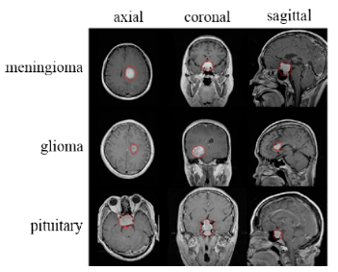
\includegraphics[scale=1.7]{dataset_des.png}
    \caption{Pictorial representation of types of data in the MRI dataset}
    \label{fig:dataset_img}
\end{figure}

\begin{table}[ht]
    \centering
    \begin{tabular}{|c|c|c|c|c|}
        \hline
        Datset & Meningioma & Glioma & Pituitary & No tumor \\
        \hline
        Training & 822 & 826 & 827 & 395 \\
        Testing & 115 & 100 & 105 & 74 \\
        \hline
    \end{tabular}
    \caption{Detailed analysis of distribution of MRI dataset}
    \label{tab:dataset_distribution}
\end{table}

\section{Data visualisation}\label{sec:3.2}
A detailed analysis and visualisation of dataset is performed before employing any machine learning or deep learning methods for classification of tumor from brain MRI images. The images are plotted in python programming language using matplotlib library which is extensively used to plot graphs and images. First nine images from the training dataset for each class is ploted for visualisation of dataset for each class. A better understanding of quality and resolution of images is drawn by this analysis. Moreover a deeper understanding of each type of data and its representation for each class is achieved by this method. A detailed qualitative analysis of meningioma tumors is illustrated in Figure \ref{fig:meningioma}. Meningioma is the most common primary brain tumour, accounting for more than 30\% of all brain tumours. The three outer layers that surround and protect the brain immediately under the skull, the meninges, are where these tumours develop. Diagnoses of meningioma are seen more commonly in women than in men. A significant portion of meningiomas, about 85\%, are noncancerous and distinguished by their slow development. Although the majority of meningiomas are benign, some of them might persist and reappear after therapy. However, their growth may have an adverse effect on the brain, leading to a variety of impairments like poor eyesight, hearing, memory loss, and even convulsions. Meningioma incidence tends to increase with age, and because of the slow growth of these tumours, symptoms gradually worsen over time.

\begin{figure}
    \centering
    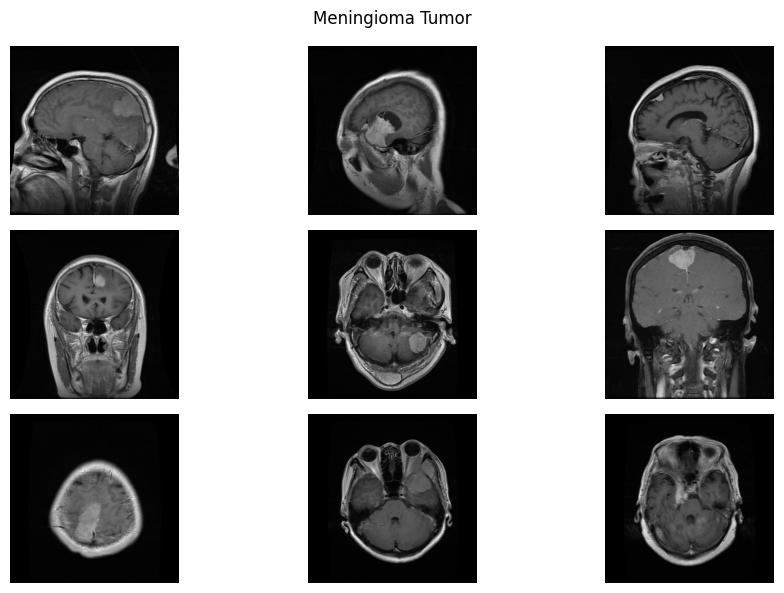
\includegraphics[scale=0.7]{Meningioma.png}
    \caption{Qualitative analysis of Meningioma tumor from the kaggle dataset.}
    \label{fig:meningioma}
\end{figure}

A detailed qualitative analysis of Glioma tumors is illustrated in Figure \ref{fig:Glioma}. Gliomas the most significant primary brain tumour denotes its origin inside the brain itself and ranks third among all brain tumours in terms of frequency. Sadly, it also holds the distinction of being the most deadly. Glioblastoma is a rare cancer that affects the brain. Every year, about 15,000 new cases are discovered, with typical survival times of 11 to 15 months. Gliomas are the most common kind of adult brain tumour, accounting for 78\% of malignant brain tumours.

\begin{figure}
    \centering
    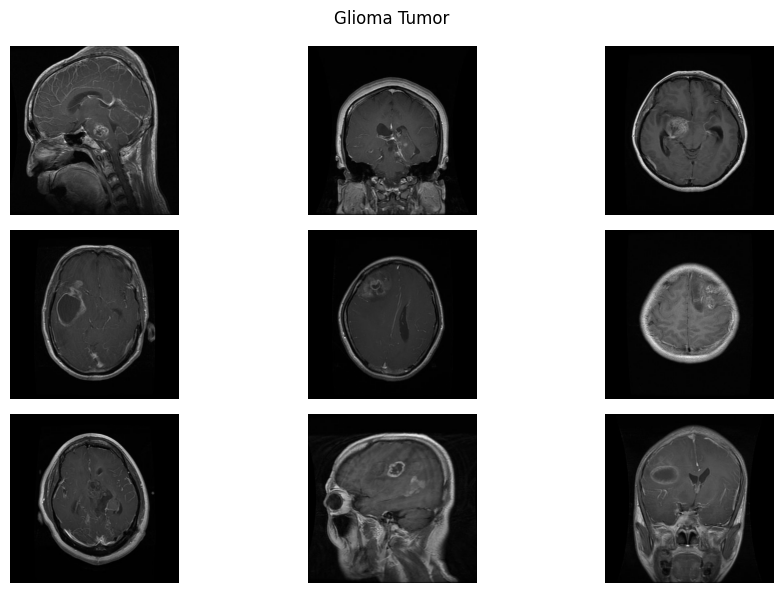
\includegraphics[scale=0.7]{Glioma.png}
    \caption{Qualitative analysis of Glioma tumor from the kaggle dataset.}
    \label{fig:Glioma}
\end{figure}

A detailed qualitative analysis of Pituitary tumors is illustrated in Figure \ref{fig:Pituitary}. The most frequent intracranial tumours are pituitary, which are followed by gliomas, meningiomas, and schwannomas. Pituitary often have benign qualities and develop at a relatively slow rate. It's important to understand that the chance of malignant pituitary tumours spreading to other bodily areas is quite unlikely. Adenomas are undoubtedly the most common pituitary disorders. These growths can appear in youngsters, however they are often identified in people in their 30s or 40s. Fortunately, a large percentage of malignant tumours may be successfully treated.

\begin{figure}
    \centering
    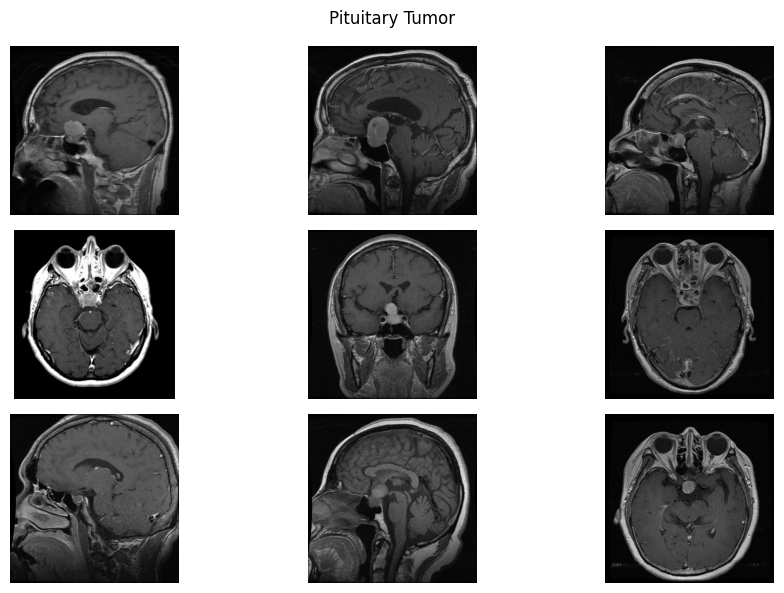
\includegraphics[scale=0.7]{Pituitary.png}
    \caption{Qualitative analysis of Pituitary tumor from the kaggle dataset.}
    \label{fig:Pituitary}
\end{figure}

A detailed qualitative analysis of No tumors is illustrated in Figure \ref{fig:no_tumor}. These images with no tumors are included into dataset such that the model also learns about 'no tumor' condition and can flag such conditions. Moreover it is important to also make the model learn about false images (with no tumor) such that a healthy regular brain MRI images is feed into the convolutions of the deep learning model.

\begin{figure}[h]
    \centering
    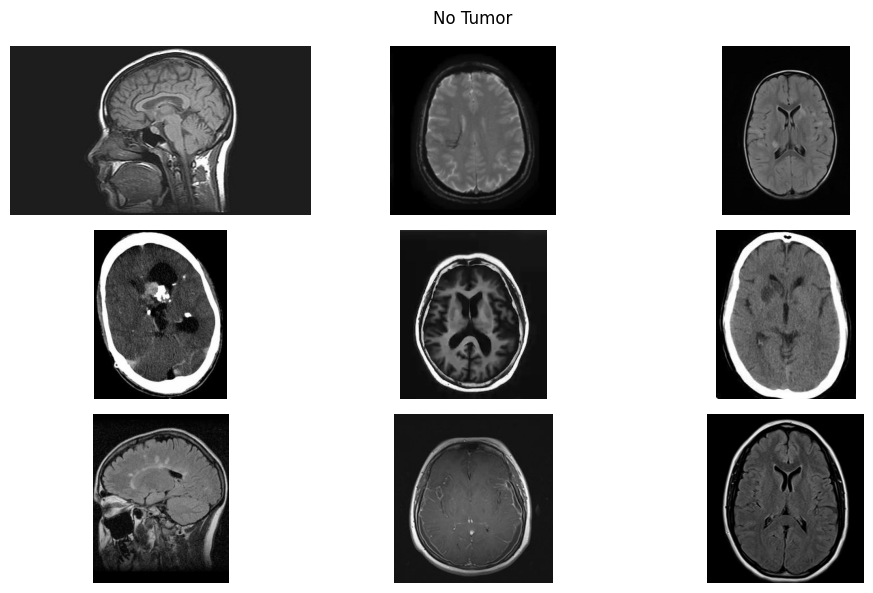
\includegraphics[scale=0.7]{no tumor.png}
    \caption{Qualitative analysis of No tumor images from the kaggle dataset.}
    \label{fig:no_tumor}
\end{figure}


\section{Data preparation}\label{sec:3.3}
Preparation of data for training the model is one of the most important and critical step. It is challenging to prepare data for training and testing of model due to limitation of deep learning models. These models cannot directly learn from an RGB images as human being, although they divide an image into specific sized matrix of pixels and based on intensity of RGB channels it learns about the patterns and features of an image. Therefore we need to convert the RGB images into a pixel matrix. For this study I have initialised the images as list variables from the RGB channel for each set of data (Training and test dataset). Our proposed algorithm have investigated each image path from all the classes of brain tumor in both the set of images (training and test) and have extracted pixel value from each image and appended that into the list. Furthermore these list for training and test set are converted to numpy array which is acceptable by most of the deep neural network. Arrays are easier and faster to process therefore most of the deep learning models take input of images as an array format. 

Henceforth the conversion of images into array of lists of pixel values, I have amalgamated the feature set and target set for both the train and test data, this is done to shuffle the dataset and bring more generalisation to the dataset. Equation \ref{eq:x_train} and \ref{eq:y_train} shows the amalgamation of features (X) and targets(y) from both the sets. 
\begin{equation}
    X\_train = X\_train + X\_test
    \label{eq:x_train}
\end{equation}

\begin{equation}
    y\_train = y\_train + y\_test
    \label{eq:y_train}
\end{equation}

The pixel data for both target and features are shuffled by a python library, 'shuffle'. Thereafter the train and test data is split in the ratio of 80:20 respectively. Moreover the target data is also converted into categorical type as the it is computationally faster to process a categorical value as compared to a decimal value. Deep learning models are highly computationally costly and requires a lot of time to process a forward and back propagation for each epochs, and the use of categorical target values can decrease the training time to certain extent.

\section{Defining model}\label{sec:3.4}
I have used two different models in this study: 1. MobileNet and 2. InceptionNet V3. Performance is evaluated for each model to monitor its effectiveness  for classification of brain MRI images to detect tumors, considering the fact that all the hyperparameters for both the model are kept similar to fairly compare the effectiveness of the model. I have modified both the pre existing deep learning models such that it's performance for classification of image is enhanced. The architecture of both the modified pre\-existing models are discussed in subsequent subsections:

\subsection{Model 1: MobileNet}\label{sec:3.4.1}
A CNN based model that is often used for picture categorization is MobileNet \cite{khasoggi2019efficient}. The MobileNet architecture's requirement for far fewer computing resources than traditional CNN models is a major advantage. This feature makes it suitable for use on mobile devices and PCs with constrained processing power. The MobileNet model is a simplified framework with a convolutional layer that uses two controllable features to successfully balance parameter accuracy and latency to distinguish fine details. Additionally, the MobileNet concept has a benefit in terms of reducing network size. A small handful of characteristics are used to great effect in the MobileNet architecture. MobileNet has a depth-wise architecture in terms of structure. It centres on several abstraction layers that evaluate issue complexity at various levels and are made up of numerous convolutions that make up a quantized arrangement. Point-wise complexity is represented by the symbol 1 $\times$ 1. Structures are integrated using abstraction layers intended for depth, whereas point-wise channelling uses a typical ReLU (rectified linear unit). The resolution multiplier parameter, represented by $w$, is introduced to reduce the dimensionality of input images and internal representations across layers. This parameter guarantees a consistent reduction in the size of the input picture as well as the internal representation of each layer.

A filter with dimensions $F_s \times F_s$ interacts with the typical vector map, which has $F_m \times F_m$ dimensions. The output variable is denoted by the letter $q$, whereas the input variable is represented by the letter $p$. The variable $c_e$ contains the cumulative computational effort inside the fundamental abstraction layers of the design. This may be assessed using the equation below:

\begin{equation}
    c_e = F_s \cdot F_s \cdot w \cdot \alpha F_m + w \cdot  p \cdot \alpha F_m \cdot  \alpha F_m
\end{equation}

The multiplier value depends on the situation, and in the context of experimental analysis for classifying skin diseases, the multiplier$w$ is investigated in the range of 1 to n. The resolution multiplier variable $\alpha$ stays at 1. Equation (2), which is presented below, may be used to calculate computation effort using the variable $cost_e$:

\begin{equation}
    cost_e = F_s \cdot F_s \cdot w \cdot p \cdot F_m \cdot F_m
\end{equation}

The depletion parameter, indicated as $d$, which is determined using the Equation given above, constrains the introduced model's ability to integrate depth and point wise convolutions.
\begin{equation}
    d = \frac{F_s \cdot F_s \cdot w \cdot \alpha F_m + w \cdot  p \cdot \alpha F_m \cdot  \alpha F_m}{F_s \cdot F_s \cdot w \cdot p \cdot F_m \cdot F_m} = \frac {c_e} {cost_e}
\end{equation}

Depending on the situation, the two hyper-parameters width multiplier and resolution multiplier are crucial for optimising the window size for accurate predictions. The picture input size for our suggested model is set at $224 \times 224 \times 3$. The image's height and width are indicated by the first two numbers $(224 \times 224)$, which both need to be more than 32. The third value denotes the presence of three input channels in the picture. 32 filters with a size of $3 \times 3 \times 3 \times 32$ are used in the suggested design. The core concept of MobileNet designs is to replace complex convolutional layers. Every layer in this method is made up of a $3 \times 3$ convolutional layer that analyses the input data, followed by a $1 \times 1$ pointwise convolutional layer that combines the filtered parameters to generate a novel element, as shown in Figure \ref{fig:mobile_net_arch}. With this method, the model will be simplified and run more quickly than with traditional convolutional models.

\begin{figure}[h]
    \centering
    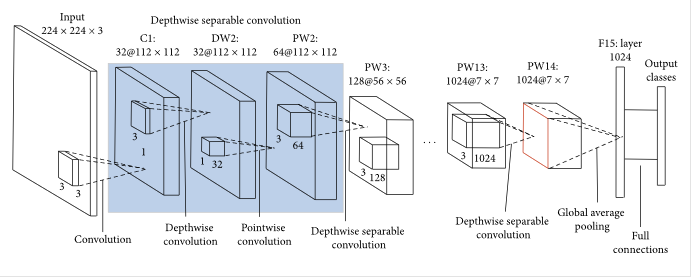
\includegraphics[scale=0.6]{mobile_net_arch.png}
    \caption{Architecture of Mobile Net.}
    \label{fig:mobile_net_arch}
\end{figure}



As mentioned above, I have modified the architecture of both the models by adding last few layers into their original architecture which have enhanced their performance for classification. I have added a Global average pooling 2D layer at the end of MobileNet which is used to converge the learnt features and patterns about the image by MobileNet. Moreover, I have used global average pooling layer as it can converge the features without losing any key features which are usually lost in case of Max pooling layer as it takes the maximum pixel value for a given pool which tends to produce wrong output for edge sensitive images like brain MRI image. Global Average Pooling also preserves the global and edge features for the image. Thereafter we have added a dense layer into the modified architecture, it is used for classification of tumors, as all the features and patterns are extracted by the MobileNet and the pooling layer helps to converge all these features together before the output layer. Softmax activation function is used to activate the neurons with maximum probability of classification. 80x80 sized brain MRI images is passed into MobileNet architecture for classification of tumors. The MobileNet model was initialized with initial weights by pre trained weights from imagenet, initialization of weights helps the model to evenly distribute the gradients and fastens the learning process as the weights are initialised as the trained weights from imagenet. A total of 3,232,964 parameters are used in this model for training the model, where 4,100 are the trainable parameters and rest 3,228,864 are the non-trainable parameters which are used in the framework of existing deep learning model. 

Our first model have used Adam as an optimizer to update the weight and biases of the network. Adam helps in generalisation thereby preventing over fitting of the model. It also helps the model learn correct set of weight and biases very quickly as its can quickly optimize the weights and baises to optimum set. Therefore it can achieve the desired score of accuracy with less epochs which end up saving computational time and resources for each model. Moreover, the Adam optimizer smoothens the gradient and thereby helps in generalisation of the model. Categorical cross entropy is used as the loss function for this model as we are using categorical target value thereby its is important to used this loss function as it will effectively calculate loss and penalise heavily for wrong set of weights and baises, thereby helping the model to learn effectively and quickly without exploding or vanishing the gradients. The model employs 'accuracy' as the metrics for calculation of loss, as our fundamental goal is to increase the accuracy of the model for classification of tumor. Penalising the model to increase the accuracy of the classification in each back propagation helps the model aim for correction of weights and baises in order to achieve high score for accuracy. 

Validation set is generated during training the model. 10\% of training data is selected at random for validation of model, validation set is important to evaluate the performance of the model while training. At the end of each epoch, the model is validated by validation set to check performance of the model, moreover the validation set is unseen dataset therefore it prevents the model from over fitting and helps the model learn from generalised data after each epoch. A batch size of 32 is considered for training of our first model, a smaller batch size will help the model learn key features from the image, it might increase the computational usage and timing but it helps the model learn about minute features from the images. The modified model of MobileNet is trained for 10 epochs. 


\subsection{Model 2: InceptionNet V3}\label{sec:3.4.2}
The GoogleLeNet network is a convolutional neural network (CNN), which was first introduced by Google in 2014. It adopts the Inception network's architectural design, which not only results in a decrease in network parameters but also makes it possible to improve network depth. This makes it a very popular option for tasks involving picture categorization. The Inception network topology, which forms the GooLeNet network's core, is also known as the Inception network \cite{abadi2016tensorflow}. Inception v1 (2014), Inception v2 (2015), Inception v3 (2015), Inception v4 (2016), and Inception-ResNet (2016) are the most prominent versions of Google LeNet. The Inception module typically encompasses three distinct convolution sizes along with a maximum pooling layer. After the convolution operation, the network's previous layer output is combined across channels, followed by nonlinear fusion. This approach enhances network expressiveness, adaptability to varying scales, and helps mitigate overfitting. 

The structure of the Inception network is illustrated in Figure \ref{fig:inception_net}. Inception v3, primarily an architecture developed by Keras, is pretrained on the ImageNet dataset. By default, it accepts images of size 299x299 with three color channels. The Inception v3 network structure utilized in this study is depicted in Figure \ref{fig:inception_v3}. Convolution kernel splitting, which divides larger convolutional operations into smaller components, is a method used by the Inception v3 network architecture in contrast to its forerunners (Inception v1 and v2). A 3x3 convolution, for instance, is split into two steps: a 3x1 and then a 1x3 convolution. The extraction of spatial information is improved while also speeding up network training because to this splitting strategy's reduction in the number of parameters. Inception v3 simultaneously improves the Inception network's module by optimising it over three different grid regions of varying sizes (35x35, 17x17, and 8x8), as seen in Figure \ref{fig:inception_mod}.

\begin{figure}[h]
    \centering
    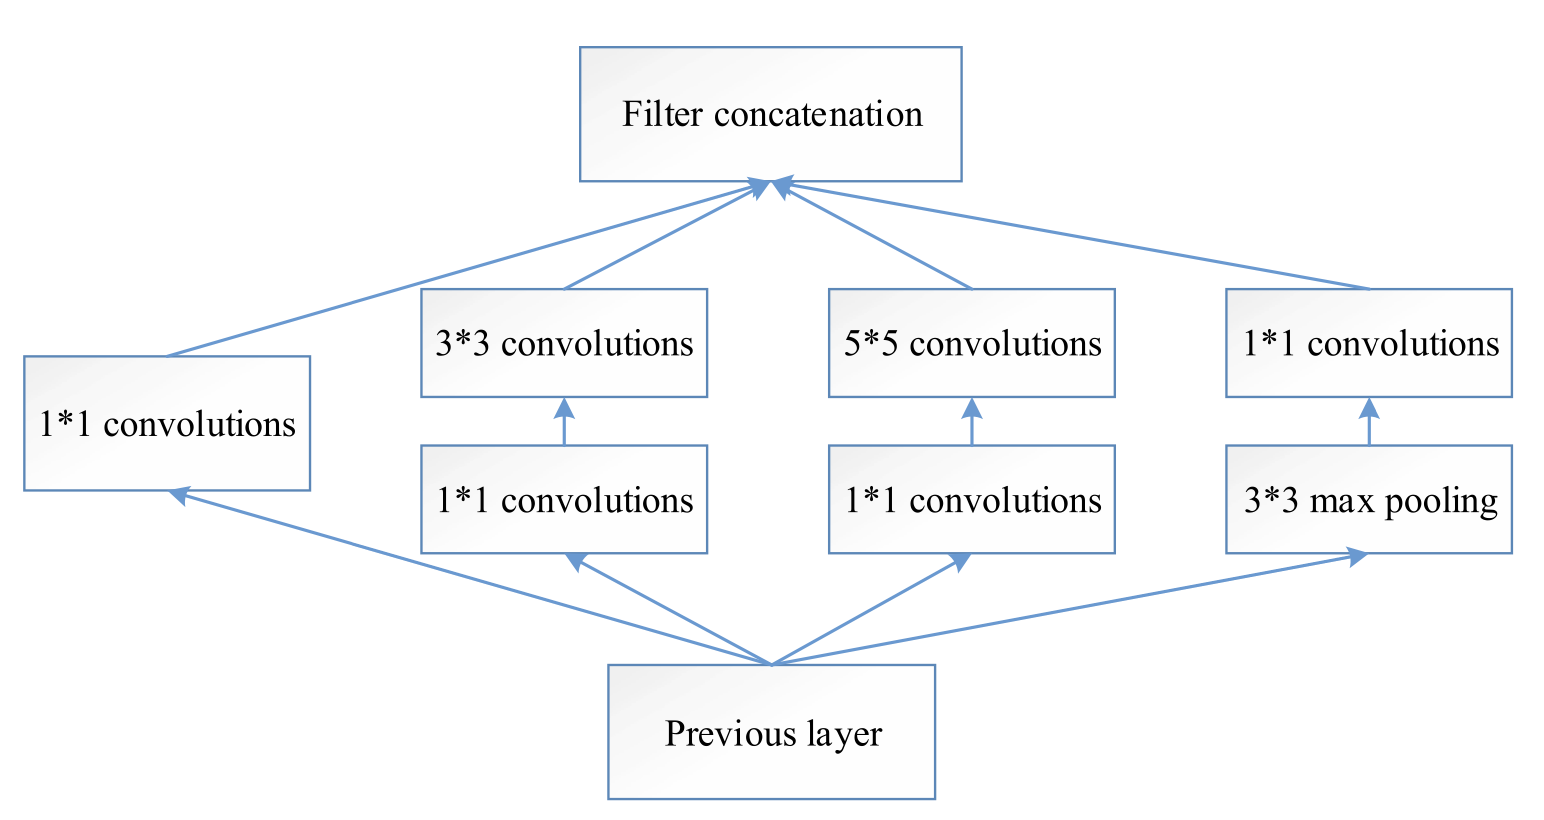
\includegraphics[scale=0.5]{Inception_network.png}
    \caption{Architecture of inception network}
    \label{fig:inception_net}
\end{figure}

\begin{figure}[h]
    \centering
    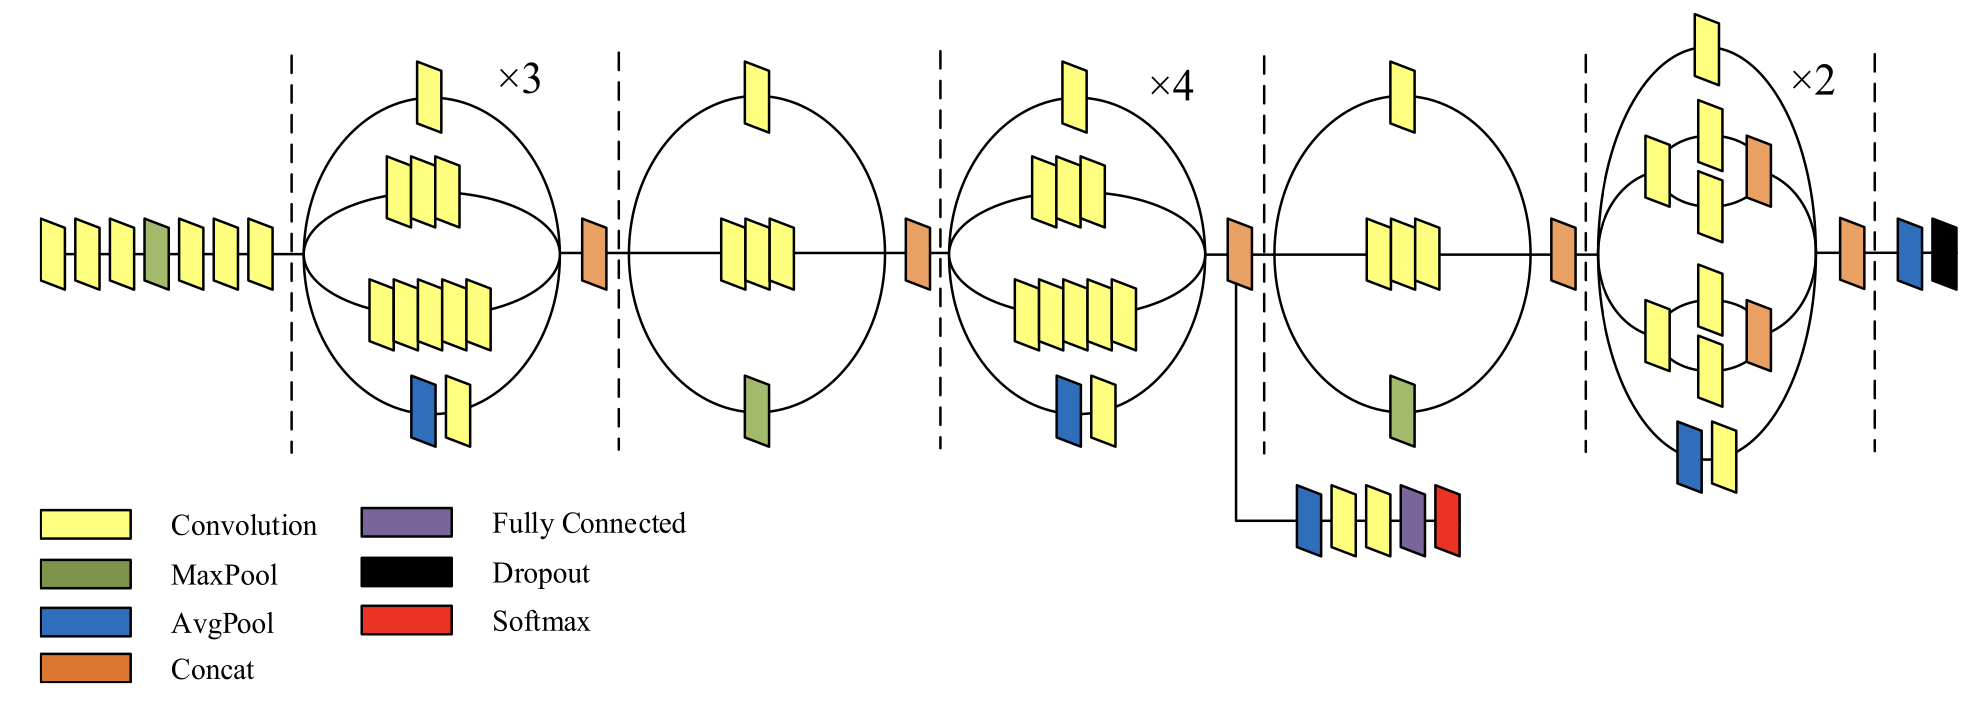
\includegraphics[scale=0.4]{Inception v3.png}
    \caption{Architecture of Inception Net v3 network}
    \label{fig:inception_v3}
\end{figure}

\begin{figure}[h]
    \centering
    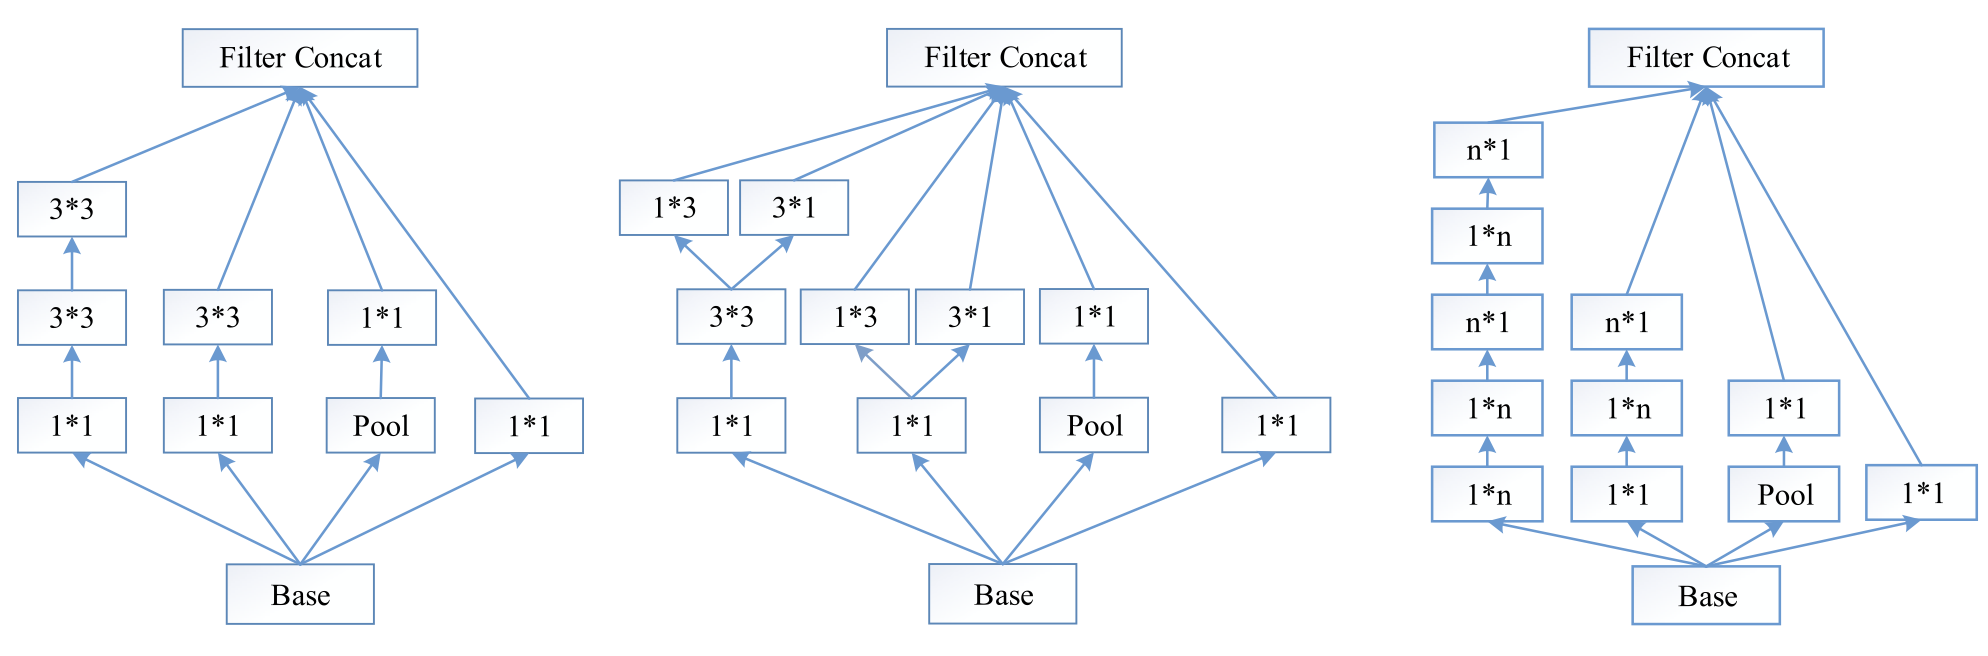
\includegraphics[scale=0.4]{Inception module.png}
    \caption{Architecture of Inception module in inception network}
    \label{fig:inception_mod}
\end{figure}


Similar to our first model, we have added a Global average pooling layer and a  output layer to original architecture of InceptionNet. We have used the pre trained weights from imagenet to initialise the initial weights of InceptionNet. The pooling layer is added to extract the key features which is generated by the InceptionNet model. Thereafter a dense layer is used to classify the four different tumors based on pictorial and pattern differences. Hyperparameters used in this model are same as the first model, i.e. we have used Adam as the optimizer, with categorical cross entropy as loss function and accuracy metrics is used along with a similar batch size of 32 and for 10 epochs. All the hyperparamters are kept similar as we want to evaluate the performance of MobileNet with InceptionNet V3 under similar hyperparamatric condition. Moreover we have splitted the validation set from the training set at an ratio of 90:10, which is similar to the first model using MobileNet.


A detailed result and analysis is shown in next chapter where we have discussed about the evaluation parameters and have compared the performance both the models for classification of tumors from brain MRI images.

\chapter{Results and discussion}\label{ch:4}
A detailed result analysis is drawn in this chapter which measures the performance of both the models based on architecture of MobileNet and InceptionNet V3. Additionally we have also discussed about the Parameters for evaluation in the chapter. 

\section{Parameters for evaluation}\label{sec:4.2}
The performance of classification of brain tumor is evaluated based of the predicted value and actual value. Figure \ref{fig:con_mat_eg} represents a confusion matrix with actual and predicted value. In a multi class classification an actual subject (class of tumor) is considered as positive value where as all the images from other classes are considered as negative when we are classifying for that class. For example, when the classification result is generated for Meningioma tumor, it is considered as positive value while all the other classes (Glioma tumor, Pituitary tumor and no tumor) are considered as negative values, similary for other classes the value for positive and negative changes. The performance of each class is classified by the values of: 

1. True positive - When an actual positive value is classified/predicted as a positive value then it is termed as true positive.

2. False Negative - When an actual positive value is wrongly classified as negative value.

3. False Positive - When actual negative value is wrongly classified as positive value.

4. True Negative - When an actual negative value is classified as negative value.

\begin{figure}
    \centering
    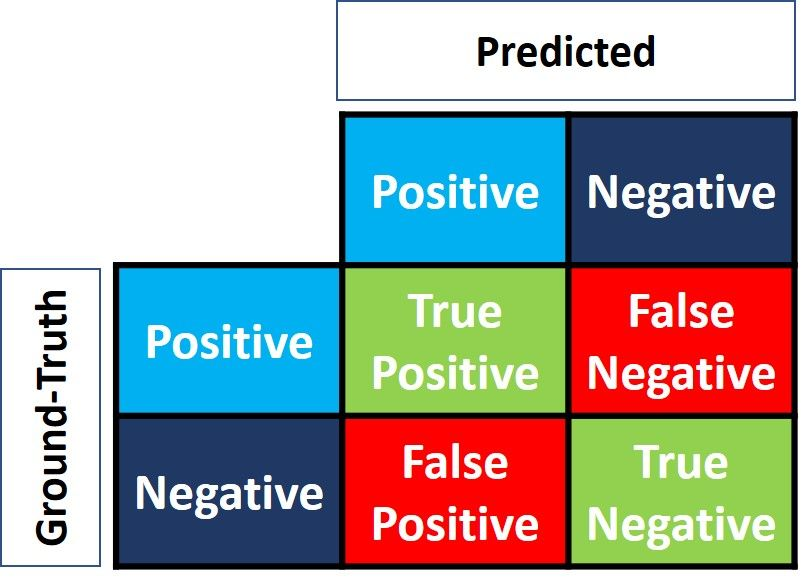
\includegraphics[scale=0.3]{Fig01.jpg}
    \caption{Pictorial representation of confusion matrix for classification of each class of tumor}
    \label{fig:con_mat_eg}
\end{figure}

The following evaluation metrics are used to calculate the performance of the model: 

1. Precision - A measure of precision counts how many reliable positive forecasts were made. It is calculated by dividing the total number of positively anticipated cases by the number of properly predicted positive occurrences.
\begin{equation}
    Precision = \frac{TP}{TP+FP}
\end{equation}

2. Recall -  Recall is a statistic that measures how many correct positive predictions were produced out of all possible positive predictions. Recall provides information about potential missed positive predictions as opposed to precision, which concentrates only on the accurate positive predictions among all positive predictions.
\begin{equation}
    Recall = \frac{TP}{TP+FN}
\end{equation}

3. F1 Score - Classification accuracy is widely used because it can be used to summarise the performance of a model using a single statistic. The F-Measure provides a method for combining recall and accuracy into a single statistic that encompasses both elements. Precision and recall do not provide a thorough insight when viewed separately. It is possible to have excellent recall while having poor accuracy, or vice versa. The F-measure overcomes this by offering a single score that takes into account both factors.
\begin{equation}
    F1 = \frac{2*Precision*Recall}{Precision+Recall} = \frac{2*TP}{2*TP+FP+FN}
\end{equation}

4. Accuracy - It is the measure of the overall performance of the model based on the outcome for actual positive value.
\begin{equation}
    Accuracy = \frac{TP+TN}{TP+TN+FP+FN}
\end{equation}

\section{Results}\label{sec:4.3}
The performance of both the modified deep learning model is discussed in this section. Both the models are executed for 10 epochs with a similar set of hyper parameters. Pictorial representation of training and validation accuracy is shown in figure \ref{fig:m1_acc}. The graph represents the increase in accuracy for training and validation set, whereas there is a decrease in validation score after the 8 epoch of the Mobile net model, it is evitable that if we would have executed the model for more than 10 epochs the validation score would have been increase as the model was learn to adjust its weight and biases for generalised dataset. It is also visible that the learning curve for the validation set often decreases at certain intervals and then shows an gradual progression which indicates that a higher epoch value will increase the overall accuracy of the model. Figure \ref{fig:m1_loss} portrays the loss after each epoch by the training and validation set. It indicates a gradual decrease in loss of the model which is a good indication of accurate optimisation of model. 

\begin{figure}[h]
    \centering
    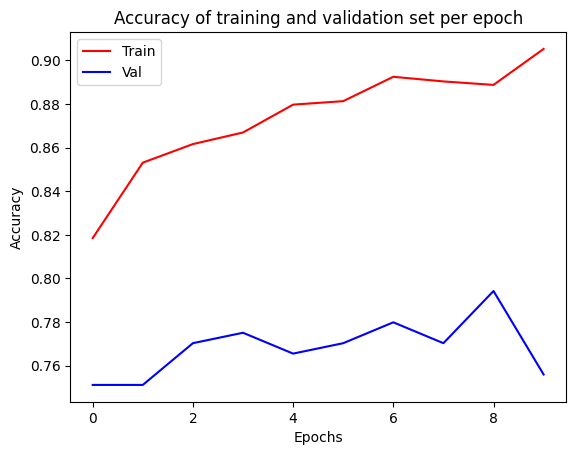
\includegraphics[scale=0.6]{Model1_acc.png}
    \caption{Pictorial representation of accuracy for each epoch by Model 1.}
    \label{fig:m1_acc}
\end{figure}

\begin{figure}[h]
    \centering
    \includegraphics[scale=0.6]{Model1_loss.png}
    \caption{Pictorial representation of loss for each epoch by Model 1.}
    \label{fig:m1_loss}
\end{figure}

Figure \ref{fig:m2_acc} plots the accuracy for each epochs by model 2: Inception net V3. It shows the accuracy of the model increases exponentially and if the model would have been trained for more epochs the accuracy mark could have touched a significant score. Similarly, the loss of the of the model is represented in  Figure \ref{fig:m2_loss}, which shows an exponential loss by both training and validation set. Both the figures for model 2 shows an intermixing of blue and red lines (Training and validation respectively) which shows that the model is well generalised and it is not over fitting its self thereby preventing the conditions for exploding gradient. 

\begin{figure}[h]
    \centering
    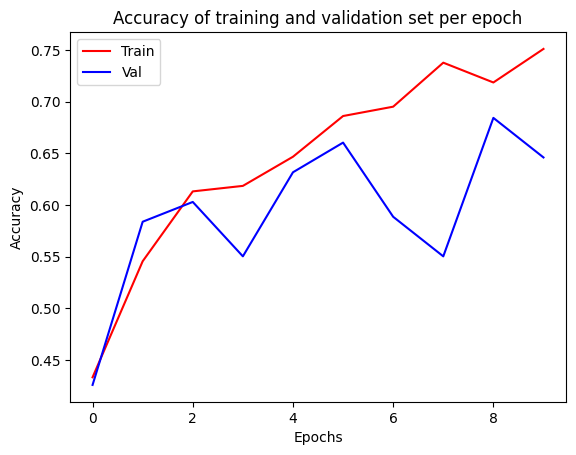
\includegraphics[scale=0.6]{Model2_acc.png}
    \caption{Pictorial representation of accuracy for each epoch by Model 2.}
    \label{fig:m2_acc}
\end{figure}

\begin{figure}[h]
    \centering
    \includegraphics[scale=0.6]{Model2_loss.png}
    \caption{Pictorial representation of loss for each epoch by Model 2.}
    \label{fig:m2_loss}
\end{figure}

Table \ref{tab:perf_acc} shows the accuracy of each model for training, test and validation dataset. It is noticeable that the training accuracy for mobile net is 90.53\% which is undoubtedly outstanding accuracy score for medical vision. It shows that the modified mobilenet is able to learn the features during its training phase to a great extent. Similarly, we can see an accuracy score of 76\% and 75.60\% for test and validation data which shows that the model also performs well with holdout dataset as the weight and baises where not trained for these datasets, it shows that the model is generalised properly and it does not have a steep gradient. Moreover the InceptionNet V3 model produces an accuracy score of 75.09\% for training dataset and 63\% and 64.59\% on test and validation dataset respectively. It is clear that the MobileNet architecture performs better than  InceptionNet V3 model it is due to the dense layer of mobilenet architecture. Moreover the training speed for mobile net was faster than inception net model, therefore I can conclude my preference of model for classification of brain tumor. 

\begin{table}[h]
    \centering
    \begin{tabular}{|c|c|c|c|}
     \hline
    Model  & Train & Test & Validation  \\  \hline
    MobileNet & 90.53\% & 76.00\% & 75.60\% \\
    InceptionNet V3 & 75.09\% & 63.00\% & 64.59\% \\
    \hline
    \end{tabular}
    \caption{Comparison of accuracy for both the models on train, test and validation dataset.}
    \label{tab:perf_acc}
\end{table}

A detailed analysis is shown in table \ref{tab:model1} where the performance of model 1 is discussed in detail. It shows the precision for classification of pituitary tumor is highest among other classes. Other metrics such as recall and f1 score is also high for pituitary tumor class. Similarly, a detailed analysis is performed for model 2 for classification for each class in table \ref{tab:model2}

\begin{table}[h]
    \centering
    \begin{tabular}{|c|c|c|c|}
     \hline
    Tumor  & Precision & Recall & F1 score  \\  \hline
    Meningioma tumor & 0.70 & 0.60 & 0.64 \\
    No tumor & 0.87 & 0.69 & 0.77 \\
    Glioma tumor & 0.64 & 0.80 & 0.71 \\
    Pituitary tumor & 0.87 & 0.91 & 0.89 \\
    \hline
    \end{tabular}
    \caption{Performance evaluation metrics for Model 1}
    \label{tab:model1}
\end{table}


\begin{table}[h]
    \centering
    \begin{tabular}{|c|c|c|c|}
     \hline
    Tumor  & Precision & Recall & F1 score  \\  \hline
    Meningioma tumor & 0.66 & 0.50 & 0.57 \\
    No tumor & 0.50 & 0.78 & 0.61 \\
    Glioma tumor & 0.77 & 0.40 & 0.52 \\
    Pituitary tumor & 0.65 & 0.87 & 0.74 \\
    \hline
    \end{tabular}
    \caption{Performance evaluation metrics for Model 2}
    \label{tab:model2}
\end{table}


If the image size was increase to 224x244, which is generally the size of pre-trained weights from imagenet then the weights could have been generalised properly and thereby would have enhanced the accuracy score. As the images are resized to 80x80 pixels the quality of image is deteriorated thereby effecting the training process. Therefore a use of high resolution image would add to the accuracy score. Moreover, if the number of epochs would have been more than 100 instead of 10, the model could have learnt more features and would have 
smoothen the gradients and thereby result in high score for accuracy. It is also noticeable that more fine tuning and experimentation with hyper parameters would fetch enhance results for classification of brain tumor.


\chapter{Conclusions}\label{ch:concl}
Medical vision is a vital domain and selection of perfect model is critical. Both the modified model for classification of brain tumor have performed well and have more potential to improve accuracy of classification. In Model 1 we have modified the original model of Mobile net and have achieved an accuracy of 76\% for test data. Moreover, model 2, where we have modified the original architecture of Inception Net V3 achieves 63\% accuracy score. After a detailed analysis of performance by both the models, I can conclude that for my further research and investigation on classification of brain tumor I will select and move forward with mobile net architecture. If we would have used the maximum possible resolution of images for training and testing then the model would have produced enhanced outcome. Moreover increasing the number of epochs would significantly increase the accuracy of the model. For my future work, in the domain of medical vision for classification of brain tumor from brain MRI images, I would employ Mobile net model with high resolution of input images and for highers epochs. I would also tune the hyper parameters to produce enhanced results for classification. 



% Comment the following THREE lines if you do NOT have an Appendix
\appendix
\chapter{Appendix: Code}
\"Identification of brain tumour from brain MRI image using machine learning techniques.ipynb

\#Downloading data from Kaggle

\!pip install opendatasets

import opendatasets as od

od.download("https://www.kaggle.com/datasets/sartajbhuvaji/brain-tumor-classification-mri")

\# Setting up train and testing paths

training\_path = 'brain-tumor-classification-mri/Training'

test\_path = 'brain-tumor-classification-mri/Testing'

\# Importing libraries

import os

import cv2

import numpy as np

import matplotlib.pyplot as plt

import keras

import tensorflow as tf

from sklearn.model\_selection import train\_test\_split

from sklearn.utils import shuffle

from keras.models import Model

from keras.layers import Dense, Dropout, Input, GlobalAveragePooling2D

from tensorflow.keras.applications import MobileNet

from tensorflow.keras.applications import InceptionV3

from tensorflow.keras.callbacks import EarlyStopping

from sklearn.metrics import classification\_report,confusion\_matrix

\#Data visualisation

\# Plotting the images for each class in training and test dataset

def plot\_images(path, title):

  list\_path=os.listdir(path)
  
  plt.figure(figsize=(10,6))
  
  plt.suptitle(title)
  
  for i in range(1,10):
  
    plt.subplot(3,3,i)
    
    img=plt.imread(os.path.join(path,list\_path[i]))
    
    plt.imshow(img)
    
    plt.axis('off')
    
  plt.tight\_layout()

\# Checking class name for training dataset, it is same for test data as well

class\_name = os.listdir(training\_path)

class\_name

\# Plotting image for Meningioma tumor

plot\_images(training\_path+'/'+class\_name[0], 'Meningioma Tumor')

plot\_images(training\_path+'/'+class\_name[1], 'No Tumor')

plot\_images(training\_path+'/'+class\_name[2], 'Glioma Tumor')

plot\_images(training\_path+'/'+class\_name[3], 'Pituitary Tumor')

\#Pre-processing of data

\# Setting image size to resize all the image to specific size, it will help during training our model with these training dataset

image\_size = 80

\# Loading images from Train and test directories

def get\_data(path, class\_name, image\_size):
  X = []
  
  y = []
  
  for i in class\_name:
  
      folderPath = os.path.join(path,i)
      
      for j in os.listdir(folderPath):
      
          img = cv2.imread(os.path.join(folderPath,j))
          
          img = cv2.resize(img,(image\_size, image\_size))
          
          X.append(img)
          
          y.append(i)
 
  return X, y

\# Loading training images and labels from directory

X\_train, y\_train = get\_data(training\_path, class\_name, image\_size)

\# Loading test images and labels from directory

X\_test, y\_test = get\_data(test\_path, class\_name, image\_size)

print("Length of X\_train: "+ str(len(X\_train)))

print("Length of X\_test "+ str(len(X\_test)))

\# Concatenating both the training and test dataset such that we can suffle the data evenly among these datasets

X\_train = X\_train + X\_test

y\_train = y\_train + y\_test

\# Converting list to numpy array such that it will be easy for processing and model training

X\_train = np.array(X\_train)

y\_train = np.array(y\_train)

\# Shuffling the dataset for better generalisation

X\_train, y\_train = shuffle(X\_train,y\_train, random\_state=51)

\# Spliting the training and testing dataset into 80:20 ratio

X\_train,X\_test,y\_train,y\_test = train\_test\_split(X\_train,y\_train, test\_size=0.2,random\_state=51)

\# converting the decimal target values to categorical values as categorical values help is faster processing and decreasses the computational cost of the model training

def labels\_to\_categorical\_values(y, class\_name):
 
  y\_new = []
  
  for i in y:
  
      y\_new.append(class\_name.index(i))
  
  y = y\_new
  
  y = tf.keras.utils.to\_categorical(y)
  
  return y

\# Converting train labels to categorical values

y\_train = labels\_to\_categorical\_values(y\_train, class\_name)
\# Converting test labels to categorical values

y\_test = labels\_to\_categorical\_values(y\_test, class\_name)

\#Model 1: Mobile net

\'Using the pre-trained weights from imagenet to mobilenet architecture, adding a pre-trained weight
helps to learn the features of the model quickly and also helps in generalisation of model,
thereby preventing the chances of overfitting\'

mobilenet = MobileNet(weights='imagenet', include\_top=False, 

input\_shape=(image\_size,image\_size, 3))

for layer in mobilenet.layers:
    layer.trainable = False

\# Global average pooling layer and dense layer with 4 neurons are used as the output layers at the end of mobilenet architecture

x = GlobalAveragePooling2D()(mobilenet.output)

out = Dense(4, activation='softmax')(x)

model = Model(inputs=mobilenet.input, outputs=out)

\# Printing model summary

model.summary()

\# Adding callbacks for earlystopping while monitoring validation loss

callbacks=[EarlyStopping(monitor='val\_loss',patience=10)]

\# Setting hyperparameters of the model

model.compile(optimizer='Adam', loss='categorical\_crossentropy', metrics=['accuracy'])

\# Training the model for 10 epochs and 32 batch size, spliting the training data into 90:10 ratio for validation dataset

history=model.fit(X\_train, y\_train,validation\_split=0.1,epochs=10, batch\_size=32)

\# Plot history of the training to check what happens per epoch

def plot\_history(train, validation, title):
  
  plt.plot(train, color = 'r')
  
  plt.plot(validation, color = 'b')
  
  plt.xlabel("Epochs")
  
  plt.ylabel(title)
  
  plt.title(title+" of training and validation set per epoch")
  
  plt.gca().legend(('Train','Val'))
  
  plt.show()

\# Plotting training and validation accuracy

plot\_history(history.history['accuracy'], history.history['val\_accuracy'], "Accuracy")

\# Plotting training and validation loss

plot\_history(history.history['loss'], history.history['val\_loss'], "Loss")

\# Evaluating the model

pred = model.predict(X\_test)

# Conversion to pred and y\_test to decimal value from categorical value as classification report is generated based on decimal value comparision

pred = np.argmax(pred,axis=1)

y\_test\_new = np.argmax(y\_test,axis=1)

print(classification\_report(y\_test\_new,pred))

\#Model 2:Inception net

inceptionv3 = InceptionV3(weights='imagenet', include\_top=False, input\_shape=(image\_size,image\_size, 3))

for layer in inceptionv3.layers:
    layer.trainable = False

x = GlobalAveragePooling2D()(inceptionv3.output)
out = Dense(4, activation='softmax')(x)

inception\_net\_model = Model(inputs=inceptionv3.input, outputs=out)

callbacks=[EarlyStopping(monitor='val\_loss',patience=10)]

inception\_net\_model.compile(optimizer='adam', loss='categorical\_crossentropy', metrics=['accuracy'])

inception\_net\_history=inception\_net\_model.fit(X\_train, y\_train, validation\_split = 0.1, batch\_size = 32, verbose=1, epochs = 10, callbacks=callbacks)

\# Plotting training and validation accuracy

plot\_history(inception\_net\_history.history['accuracy'], inception\_net\_history.history['val\_accuracy'], "Accuracy")

\# Plotting training and validation loss

plot\_history(inception\_net\_history.history['loss'], inception\_net\_history.history['val\_loss'], "Loss")

\# Evaluating the model

pred = inception\_net\_model.predict(X\_test)

\# Conversion to pred and y\_test to decimal value from categorical value as classification report is generated based on decimal value comparision

pred = np.argmax(pred,axis=1)

y\_test\_new = np.argmax(y\_test,axis=1)

print(classification\_report(y\_test\_new,pred))


\bibliographystyle{abbrv}
\bibliography{xbib}



\end{document}

